\chapter{Industrial Test Case}
\chaptertoc{}

In the previous chapters, the validation of each essential component for the
industrial simulation was conducted. Chapter 1 provided a brief overview of the
Lattice Boltzmann Method (LBM). In Chapter 2, the thermodynamic properties and
the computation of the caloric equation from a cubic equation of state were
developed. Chapter 3 focused on the Immersed Boundary Method (IBM) and included
a comparison of three different implementation approaches.

In this chapter, we present a detailed description of the industrial test case
and the simulation of a single component, which serves as the primary focus of
this PhD work.

\section{CIXTEN Thermodynamical Cycles}

As discussed in the introduction, supercritical fluids have recently gained
significant interest due to their unique thermodynamic properties, which enable
the recovery of energy that would otherwise be lost to the atmosphere.

CIXTEN is developing a new machine designed to exploit the advantageous
properties of supercritical $\ce{CO2}$. The company is exploring two main
commercial applications:

\begin{enumerate}
    \item \textbf{Thermal enhancement}, based on the thermodynamic cycle illustrated in Fig.~\ref{}.
    \item \textbf{Electricity generation}, following the thermodynamic cycle shown in Fig.~\ref{}.
\end{enumerate}


In this work, the author focuses on the second cycle, specifically on the
thermal compressor.

To understand better the industrial configuration, a more simplified
thermodynamical cycle is showed on Fig.~\ref{fig:SimplifiedIndustrialCycle}.

\begin{figure}[htbp]
    \centering
    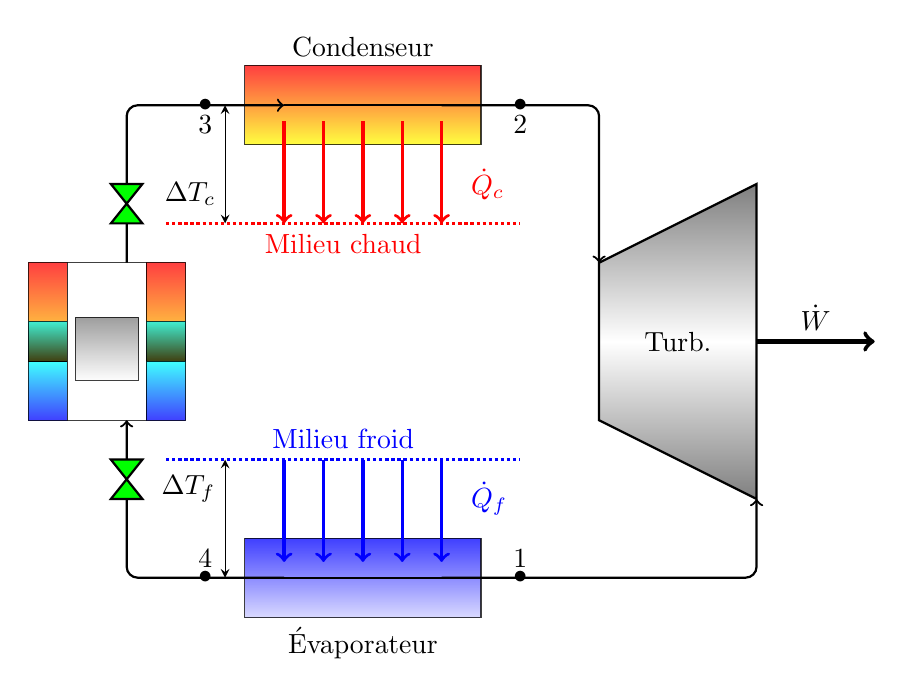
\begin{tikzpicture}[scale=1]

    %%%% SHE 
    %%%%%%%%%%%%%%%%%%% Left %%%%%%%%%%%%%%%%%%%%%%%%%%%%%%% 
    \shadedraw [top color=red,bottom color=yellow,opacity=0.75] (0.75,4.75) rectangle (1.25,6);
    \shadedraw [top color=cyan,bottom color=blue,opacity=0.75] (0.75,4) rectangle (1.25,4.75);
    \shadedraw [top color=cyan,bottom color=black,opacity=0.75] (0.75,4.75) rectangle (1.25,5.25); %Adiabatic wall

    %%%%%%%%%%%%%%%%%%%% Center %%%%%%%%%%%%%%%%%%%%%%%%%%%%%%
    \shadedraw [top color=white,bottom color=white,opacity=0.75] (1.25,4) rectangle (2.25,6);
    \shadedraw [top color=gray,bottom color=white,opacity=0.75] (1.35,4.5) rectangle (2.15,5.3); %Deplaceur

    %%%%%%%%%%%%%%%%%% Right %%%%%%%%%%%%%%%%%%%%%%%%%%%%%%%%%%% 
    \shadedraw [top color=red,bottom color=yellow,opacity=0.75] (2.25,4.75) rectangle (2.75,6);
    \shadedraw [top color=cyan,bottom color=black,opacity=0.75] (2.25,4.75) rectangle (2.75,5.25); %Adiabatic wall
    \shadedraw [top color=cyan,bottom color=blue,opacity=0.75] (2.25,4) rectangle (2.75,4.75);

    %%%%%%%%%%%%%%%%% dsd%%%%%%%%%%%%%%%%%%%%%%%%%%%%%%%%%%%%%%%%

    % Condenseur
    \shadedraw [top color=red,bottom color=yellow,opacity=0.75] (3.5,7.5) rectangle (6.5,8.5);
    \draw [thick] (4,8) -- (6,8);  % straight line instead of zigzag
    \draw (5,8.5) node [above] {Condenseur};

    % Evaporateur
    \shadedraw [top color=blue,bottom color=blue!20,opacity=0.75] (3.5,1.5) rectangle (6.5,2.5);
    \draw [very thick,blue,densely dotted] (2.5,3.5) --+ (4.5,0) node [midway,above] {Milieu froid};
    \draw [very thick,red,densely dotted] (2.5,6.5) --+ (4.5,0) node [midway,below] {Milieu chaud};

    % Arrows replacing snake decorations
    \foreach \x in {4,4.5,...,6} {
        \draw [very thick,->,blue] (\x,3.5) --+ (0,-1.3);
        \draw [very thick,->,red] (\x,7.8) --+ (0,-1.3);
    }

    \draw [blue] (6.25,3) node [right] {$\dot{Q}_f$};
    \draw [red] (6.25,7) node [right] {$\dot{Q}_c$};
    \draw [stealth-stealth] (3.25,6.5) --+ (0,1.5) node [left,near start] {$\Delta T_c$};
    \draw [stealth-stealth] (3.25,2) --+ (0,1.5) node [left,near end] {$\Delta T_f$};
    \draw [thick] (4,2) -- (6,2);  % straight line instead of zigzag
    \draw (5,1.5) node [below] {\'Evaporateur};

    % Circuit
    \draw [thick,rounded corners,->] (4,2) -- (3,2) node {$\bullet$} node [above] {4} -- (2,2) -- (2,4);
    \draw [thick,rounded corners,->] (2,6) -- (2,8) -- (3,8) node {$\bullet$} node [below] {3} -- (4,8);
    \draw [thick,rounded corners,->] (6,8) -- (7,8) node {$\bullet$} node [below] {2} -- (8,8) -- (8,6);
    \draw [thick,rounded corners,<-] (10,3) -- (10,2) -- (7,2) node {$\bullet$} node [above] {1} -- (6,2);

    % Detendeur haut
    \draw [thick,fill=green] (1.8,7) -- (2.2,7) -- (1.8,6.5) -- (2.2,6.5) -- cycle;

    % Detendeur bas
    \draw [thick,fill=green] (1.8,3.5) -- (2.2,3.5) -- (1.8,3) -- (2.2,3) -- cycle;

    % Compresseur
    \shadedraw [thick,top color=gray,bottom color=gray,middle color=white] (8,4) -- (8,6) -- (10,7) -- (10,3) -- cycle;
    \draw [ultra thick,->] (10,5) -- (11.5,5) node [midway,above] {$\dot{W}$};
    \draw (9,5) node {Turb.};

    \end{tikzpicture}
    \caption{Schematic representation of the industrial test case showing the thermal cycles and components.}
    \label{fig:SimplifiedIndustrialCycle}
\end{figure}


The Special Heat Exchanger (SHE) replaces a conventional compressor in the
s\ce{CO2} cycle. Although its schematic resembles a Brayton cycle, the SHE is
actuated by a hydraulic system and magnetic forces. It consists of two main
components: the \textbf{casing}, divided into hot, adiabatic, and cold regions,
and the \textbf{mover} (Déplaceur in french), which transfers s\ce{CO2} between
hot and cold sides. Two valves control the fluid inlet and outlet.  

The SHE cycle proceeds in four main steps, illustrated in
Figure~\ref{fig:she_cycle_simple}. Each diagram shows the relative positions of
the hot/cold regions, the mover, and the valves.

\begin{figure}[htbp]
    \centering

    %--- First row ---
    \begin{minipage}{0.45\textwidth}
        \centering
        \textbf{Step 1: Initial state.} The mover is in the hot side; both valves
        are closed. s\ce{CO2} in the cold side remains stationary.  
        \vskip 0.3cm
        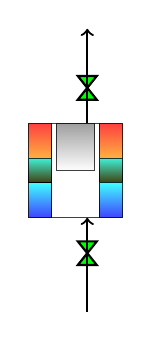
\begin{tikzpicture}[scale=0.6]
            % Hot region left
            \shadedraw [top color=red,bottom color=yellow,opacity=0.75] (0.75,4.75) rectangle (1.25,6);
            % Cold region left
            \shadedraw [top color=cyan,bottom color=blue,opacity=0.75] (0.75,4) rectangle (1.25,4.75);
            % Adiabatic wall
            \shadedraw [top color=cyan,bottom color=black,opacity=0.75] (0.75,4.75) rectangle (1.25,5.25);
            % Mover center
            \shadedraw [top color=white,bottom color=white,opacity=0.75] (1.25,4) rectangle (2.25,6);
            \shadedraw [top color=gray,bottom color=white,opacity=0.75] (1.35,5) rectangle (2.15,6);
            % Right hot/cold
            \shadedraw [top color=red,bottom color=yellow,opacity=0.75] (2.25,4.75) rectangle (2.75,6);
            \shadedraw [top color=cyan,bottom color=black,opacity=0.75] (2.25,4.75) rectangle (2.75,5.25);
            \shadedraw [top color=cyan,bottom color=blue,opacity=0.75] (2.25,4) rectangle (2.75,4.75);
            % Valves
            \draw [thick,fill=green] (1.8,7) -- (2.2,7) -- (1.8,6.5) -- (2.2,6.5) -- cycle;
            \draw [thick,fill=green] (1.8,3.5) -- (2.2,3.5) -- (1.8,3) -- (2.2,3) -- cycle;
            % Arrows
            \draw [thick,->]  (2,2) -- (2,4);
            \draw [thick,->] (2,6) -- (2,8);
        \end{tikzpicture}
    \end{minipage}\hfill
    \begin{minipage}{0.45\textwidth}
        \centering
        \textbf{Step 2:} The mover shifts to the cold side while s\ce{CO2} in the
        hot side continues to warm until 45°C.  
        \vskip 0.3cm
        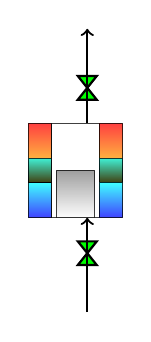
\begin{tikzpicture}[scale=0.6]
            % (Same as Step 1 but mover in cold side)
            \shadedraw [top color=red,bottom color=yellow,opacity=0.75] (0.75,4.75) rectangle (1.25,6);
            \shadedraw [top color=cyan,bottom color=blue,opacity=0.75] (0.75,4) rectangle (1.25,4.75);
            \shadedraw [top color=cyan,bottom color=black,opacity=0.75] (0.75,4.75) rectangle (1.25,5.25);
            \shadedraw [top color=white,bottom color=white,opacity=0.75] (1.25,4) rectangle (2.25,6);
            \shadedraw [top color=gray,bottom color=white,opacity=0.75] (1.35,4) rectangle (2.15,5);
            \shadedraw [top color=red,bottom color=yellow,opacity=0.75] (2.25,4.75) rectangle (2.75,6);
            \shadedraw [top color=cyan,bottom color=black,opacity=0.75] (2.25,4.75) rectangle (2.75,5.25);
            \shadedraw [top color=cyan,bottom color=blue,opacity=0.75] (2.25,4) rectangle (2.75,4.75);
            \draw [thick,fill=green] (1.8,7) -- (2.2,7) -- (1.8,6.5) -- (2.2,6.5) -- cycle;
            \draw [thick,fill=green] (1.8,3.5) -- (2.2,3.5) -- (1.8,3) -- (2.2,3) -- cycle;
            \draw [thick,->]  (2,2) -- (2,4);
            \draw [thick,->] (2,6) -- (2,8);
        \end{tikzpicture}
    \end{minipage}

    \vskip 0.5cm

    %--- Second row ---
    \begin{minipage}{0.45\textwidth}
        \centering
        \textbf{Step 3:} The hot side valve opens; s\ce{CO2} undergoes constant
        pressure heating before entering the expansion component.  
        \vskip 0.3cm
        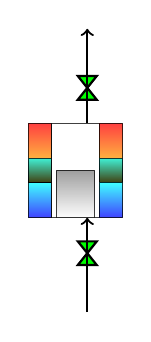
\begin{tikzpicture}[scale=0.6]
            % (Same layout, valves open)
            \shadedraw [top color=red,bottom color=yellow,opacity=0.75] (0.75,4.75) rectangle (1.25,6);
            \shadedraw [top color=cyan,bottom color=blue,opacity=0.75] (0.75,4) rectangle (1.25,4.75);
            \shadedraw [top color=cyan,bottom color=black,opacity=0.75] (0.75,4.75) rectangle (1.25,5.25);
            \shadedraw [top color=white,bottom color=white,opacity=0.75] (1.25,4) rectangle (2.25,6);
            \shadedraw [top color=gray,bottom color=white,opacity=0.75] (1.35,4) rectangle (2.15,5);
            \shadedraw [top color=red,bottom color=yellow,opacity=0.75] (2.25,4.75) rectangle (2.75,6);
            \shadedraw [top color=cyan,bottom color=black,opacity=0.75] (2.25,4.75) rectangle (2.75,5.25);
            \shadedraw [top color=cyan,bottom color=blue,opacity=0.75] (2.25,4) rectangle (2.75,4.75);
            \draw [thick,fill=green] (1.8,7) -- (2.2,7) -- (1.8,6.5) -- (2.2,6.5) -- cycle;
            \draw [thick,fill=green] (1.8,3.5) -- (2.2,3.5) -- (1.8,3) -- (2.2,3) -- cycle;
            \draw [thick,->]  (2,2) -- (2,4);
            \draw [thick,->] (2,6) -- (2,8);
        \end{tikzpicture}
    \end{minipage}\hfill
    \begin{minipage}{0.45\textwidth}
        \centering
        \textbf{Step 4:} Expansion in the turbine and cooling; the s\ce{CO2} mass
        decreases, the valve closes, and the mover resets, restarting the cycle.  
        \vskip 0.3cm
        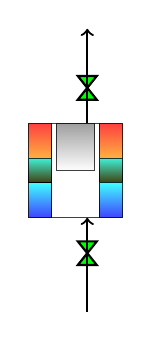
\begin{tikzpicture}[scale=0.6]
            % Same layout as above
            \shadedraw [top color=red,bottom color=yellow,opacity=0.75] (0.75,4.75) rectangle (1.25,6);
            \shadedraw [top color=cyan,bottom color=blue,opacity=0.75] (0.75,4) rectangle (1.25,4.75);
            \shadedraw [top color=cyan,bottom color=black,opacity=0.75] (0.75,4.75) rectangle (1.25,5.25);
            \shadedraw [top color=white,bottom color=white,opacity=0.75] (1.25,4) rectangle (2.25,6);
            \shadedraw [top color=gray,bottom color=white,opacity=0.75] (1.35,5) rectangle (2.15,6);
            \shadedraw [top color=red,bottom color=yellow,opacity=0.75] (2.25,4.75) rectangle (2.75,6);
            \shadedraw [top color=cyan,bottom color=black,opacity=0.75] (2.25,4.75) rectangle (2.75,5.25);
            \shadedraw [top color=cyan,bottom color=blue,opacity=0.75] (2.25,4) rectangle (2.75,4.75);
            \draw [thick,fill=green] (1.8,7) -- (2.2,7) -- (1.8,6.5) -- (2.2,6.5) -- cycle;
            \draw [thick,fill=green] (1.8,3.5) -- (2.2,3.5) -- (1.8,3) -- (2.2,3) -- cycle;
            \draw [thick,->]  (2,2) -- (2,4);
            \draw [thick,->] (2,6) -- (2,8);
        \end{tikzpicture}
    \end{minipage}

    \caption{Four-step SHE cycle showing the mover, hot/cold regions, and valve positions at each step.}
    \label{fig:she_cycle_simple}
\end{figure}


\subsection{Setup}

The simulation of SHE has the dimensions showed in
Fig.~\ref{fig:CixtenDeplaceurScheme}. In this figure we can see the principal
dimensions that are needed to make the simulations. 

The real shape of the SHE has the shape of a circular cylindrical. But due to
problems of mass loss and instabilities in the walls when this shape is used
(problems known due to interolated method used by ProLB) the shape analysed is
an square of, maintaining like that the same hydraulic diameter. 

According to CIXTEN objectives, the maximum velocity of the mover is 1 m/s. They
are only interested in one displacement movement (only one movement, not an
oscillatory one, from the hot side to the cold side).

In order to represent the mover displacement, the next equation for it's
position is imposed:

\begin{equation}
    X(t) = \mathrm{A} \times \mathrm{sin}(2 \times \pi \times f \times t) + x_0
\end{equation}

\begin{equation}
    V(t) = 2\times \mathrm{A} \times \pi \times \mathrm{cos}(\pi \times  \times f \times t) + x_0
    \label{eq:TargetVelocity}
\end{equation}

where the amplitude A = 350 mm, the frequency f = 1.0 Hz. Giving a maximal
velocity of  1 m/s for the mover.

\begin{figure}[htbp]
	\centering
	\includegraphics[width=\textwidth]{CixtenDeplaceurScheme.png}
	\caption{Scheme of the SHE with princupal dimensions used in the simulation}
\label{fig:CixtenDeplaceurScheme}
\end{figure}

For stability reasons, the mesh is uniform, and $\Delta x = \Delta y = \Delta z = $.
The time step used in the simulations is $\Delta t = $.

The mover in this simulation is going to be simulated using the IBM. To impose
the target velocity Eq.~\ref{eq:TargetVelocity} is used. Also this component is
considered as adiabatic and the T-passive condition is used. The other boundary
conditions are non slip walls. The Temperature in the hot side is 120 °C and in
the cold side the temperature is fixed to 35 °C. The supercritical $\ce{CO2}$
inside the SHE is initialised with P = 85 bar and T = 35 °C.

\subsection{Results} 
In this subsection the results of the simulations are shown. Only the setup
with the refined mesh and independent configuration is showed. 


\subsubsection{Temperature profile}

\begin{figure}[htbp]
	\centering
	\includesvg[width=\textwidth]{TVStime}%
	\caption{Temperature profile over time in the point ...}
\label{fig:TVStime}
\end{figure}

\subsubsection{Pressure profile}
\begin{figure}[htbp]
	\centering
	\includesvg[width=\textwidth]{PVStime}%
	\caption{Pressure profile over time in the point ...}
\label{fig:PVStime}
\end{figure}

\subsubsection{Global convective coefficient}

In order to determine the Global convective coefficient, a simple control volume
is analysed. The particularity of this control volume is that is constant, as
shown in ~\ref{fig:SchemeControlVolume}.

\begin{figure}[htbp]
	\centering
	\includegraphics[width=\textwidth]{SchemeControlVolume.png}%
	\caption{Temperature profile over time in the point ...}
\label{fig:SchemeControlVolume}
\end{figure}

Applying an energy conservation to this volume we have: 

\begin{equation}
    m_{\ce{CO2}} \frac{\mathrm{d}U}{\mathrm{d}t} = h \times S \times (T_h - T_{\ce{CO2}})
\end{equation}

\begin{equation}
    m_{\ce{CO2}} C_v \frac{\mathrm{d} T_{\ce{CO2}}}{\mathrm{d}t} = h \times S \times (T_h - T_{\ce{CO2}})
\end{equation}

\begin{equation}
     C_v \frac{\mathrm{d} T_{\ce{CO2}}}{T_h - T_{\ce{CO2}}} = \frac{h \times S \times \mathrm{d}t }{m_{\ce{CO2}}}
\end{equation}

\begin{equation}
    \int  \frac{C_v}{T_h - T_{\ce{CO2}}} \mathrm{d} T_{\ce{CO2}} = \int \frac{h \times S }{m_{\ce{CO2}}} \mathrm{d}t
\end{equation}

\begin{equation}
    \sum  \frac{C_v}{T_h - T_{\ce{CO2}}} \Delta T_{\ce{CO2}} =  \frac{h \times S }{m_{\ce{CO2}}} \Delta t
\end{equation}

\begin{equation}
    \sum  \frac{C_v}{T_h - T_{\ce{CO2}}} \Delta T_{\ce{CO2}} \frac{ m_{\ce{CO2}} }{\Delta t \times S}  =  h
\end{equation}


\subsubsection{Local convective coefficient}